\documentclass[11pt]{article}
% default ORG mode 
\usepackage[utf8]{inputenc}  \usepackage[T1]{fontenc} \usepackage{fixltx2e}
\usepackage{graphicx}        \usepackage{longtable}   \usepackage{float}
\usepackage{wrapfig}         \usepackage{soul}        \usepackage{textcomp}
\usepackage{marvosym}        \usepackage{wasysym}     \usepackage{latexsym}
\usepackage{amsmath}         \usepackage{amssymb}     \usepackage{color}
\usepackage{rotating}        \usepackage{hyperref}    \usepackage{xcolor} 
\usepackage{palatino}
% my customizations
\usepackage{enumitem}
\usepackage{amsthm}
\tolerance=1000
%\providecommand{\alert}[1]{\textbf{#1}}
\usepackage[top=1in, bottom=1in, left=1in, right=1in]{geometry}

\title{Dodson \& Poston Exercise VII.1.2}
\author{Peter Mao, $\ldots$}
\date{\today}

\begin{document}

\maketitle
\pagestyle{empty}

\begin{abstract}
  In-progress solution.  Feel free to add/comment/disparage.
\end{abstract}


Consider $f\colon \mathbb{R}^2 \to \mathbb{R}$ such that
\begin{align*}
  f(x,y) = 
  \begin{cases}
    |x| \exp  \bigg(
    \dfrac{(y - 2x^2)^2}
          {4x^4((y - 2x^2)^2 - x^4)}
          \bigg) &  \text{if $x^2 < y < 3x^2$} \\
    0 &\text{otherwise}
  \end{cases}
\end{align*}

\begin{itemize}
\item[\textbf{(a)}] Draw a picture of $f$.
\item[\emph{Solution}] First, notice that between the two parabolas $y = x^2$ and
  $y = 3x^2$, $f$ scales as $|x|$.  I find the non-zero part of the equation easier
  to look at with the substitution $z = x^2 \ge 0$.  Let $g(z,y)$ be the
  exponential part of $f$:
  \begin{align}
    g(z,y) &= \exp \bigg( \dfrac{(y - 2z)^2}{4z^2((y - 2z)^2 - z^2)}\bigg) \\ &=
    \exp \bigg( \dfrac{(y - 2z)^2/(4z^2)}{(y - 2z)^2 - z^2}\bigg) \label{Eqn_g},
  \end{align}
  which for any value of $z$, is defined over the open interval $(z,3z)$.  Consider
  $g(z,y)$ at some fixed value of $z$.  The independent parameter is $y$ and we can
  treat $z$ as the scaling of $y$-axis (see Figure~\ref{fig1}(i)).  The numerator of
  the exponential is a parbola in $y$ centered at $y=2z$, rising from 0 to 1/4 at
  the limits of the range.  The denominator is also a parabola rising from -1 at
  $y=2z$ to 0 at the limits of the range.

  Notice that the numerator is non-negative and the denominator is
  negative-definite, so their quotient is 0 at $y=2z$, negative everywhere else,
  and approaching $-\infty$ at the limits of the range (see Figure~\ref{fig1}(ii)).
  Thus, for any value of $z$, $g(z,2z) = 1$ and $g(z,z) = g(z,3z) =
  0$. Figure~\ref{fig1}(iii) is the $y$-direction cross section of $f$ for any non-zero
  value of $x$.

  \begin{figure}[h]
    \centerline{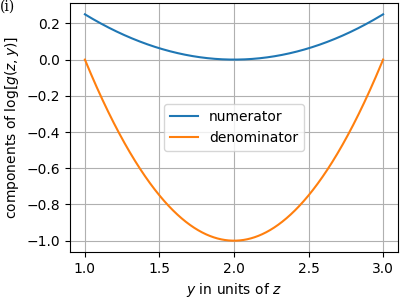
\includegraphics[width=3in]{figs/Ex.VII.1.2_fig1.png}\hspace{1em}
      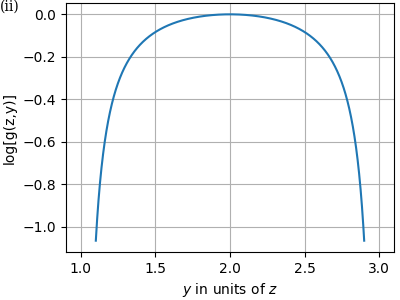
\includegraphics[width=3in]{figs/Ex.VII.1.2_fig2.png}}\\ \vspace{1em}
    \centerline{
      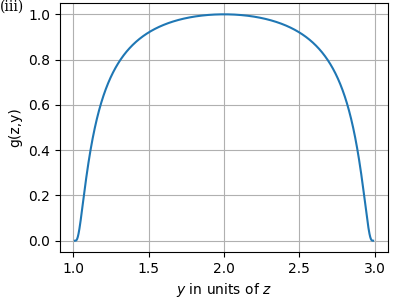
\includegraphics[width=3in]{figs/Ex.VII.1.2_fig3.png}}
    \caption{\small{\textbf{(i)} Numerator and denomintor of the argument to the
        exponential in $g(z,y)$ from Equation~\ref{Eqn_g}. \textbf{(ii)} Argument to
        the exponential in $g(z,y)$. \textbf{(iii)} $g(z,y)$: This is the shape of
        $f(x,y)/|x|$ along sections in the $y$-direction.  Notice the flatness of
        the function at the limits of its range ($y = z$ and $y = 3z$).}}
    \label{fig1}
  \end{figure}
  
  The salient features of $f$ are that it takes on a value of $|x|$ along the
  parabola $y = 2x^2$ and that it transitions smoothly to zero at $y = x^2$ and $y
  = 3x^2$.
  
\item[\textbf{(b)}]
  Show that for any vector $\vec{v} \in \mathbb{R}^2$,
  $lim_{h\to0}\frac{f(h\vec{v}) - f(0)}{h}$ exists and is zero.
\item[\emph{Solution}] Consider two classes of vectors in $\mathbb{R}^2$: Those
  with $y \le 0$ and those with $y > 0$.  In the first case, $f(h\vec{v}) = 0$, so
  the limit in question is always identically zero with no additional mental work.
  For vectors with $y > 0$, recall that $f=0$ when $y \ge 3x^2$.  Since we are
  taking $\lim_{h\to0}$, $f(h\vec{v}) = 0$ when
  \begin{align*}
    hy &\ge 3(hx)^2,
  \end{align*}
  or equivalently,
  \begin{align*}
    y  &\ge 3hx^2.
  \end{align*}
  Note that for \emph{any} positive $y$ and \emph{any} $x$, there is always an $h$
  below which this relation will hold.  Therefore, $lim_{h\to0}\frac{f(h\vec{v}) -
    f(0)}{h} = 0$ in this case as well.  Geometrically, we find that when we scale
  down any vector from the origin far enough, it will land in a region of of the
  plane where $f = 0$.

\item[\textbf{(c)}] Show that if $\vec{v_i} = (\frac{1}{i}, \frac{2}{i^2})$ we have
  $\lim_{i\to\infty}\vec{v_i} = 0$, but that in the notation of Ex.VII.1.01 if $x =
  0$ we have $d^\prime(f(x+\vec{v_i}),f(x)) = \frac{1}{i}$.
\item[\emph{Solution}] $\lim_{i\to\infty}\vec{v_i} = 0$ is obvious by
  inspection. We are given $x=0$ and$f(\vec{0}) = 0$, so
  \[d^\prime(f(x+\vec{v_i}),f(x)) = f(\vec{v_i}).\]  Since $v_y = 2v_x^2$, for any
  $\vec{v_i}$, $g(\vec{v_i}) = 1$ (the exponential part of $f$), so we have the
  desired result $f(\vec{v_i}) = |v_x| = \frac{1}{i}$.

 \newpage
  
\item[\textbf{(d)}] Find a neighborhood $N$ of the zero map $\mathbb{R}^2 \to
  \mathbb{R}$ such that
  \[
  \mathbf{A} \in N \implies \mathbf{A}\bigg(\dfrac{1}{i}, \dfrac{2}{i^2}\bigg) \ne \dfrac{1}{i}
  \]
\item[\emph{Solution}] First, note that $\mathbf{A}$ is a $1\times 2$vector
  (co-vector?) in the dual space to $\vec{v_i}$'s $\mathbb{R}^2$, so we can
  represent it as a vector or point in $\mathbb{R}^2$.  By inspection, we can see
  that for $\mathbf{A} = [1,0]$ and $\mathbf{A} = [0,i/2]$,  $\mathbf{A}\vec{v_i} =
  1/i$, so any $\mathbf{A}$ on the line passing through those two points work.
  Therefore, any neighborhood of $\mathbf{A} = [0, 0]$ that satisfies the condition
  \[
  A^y < -\frac{i}{2}(A^x - 1)
  \]
  will only contain maps that satisfies the inequality
  $\mathbf{A}\bigg(\dfrac{1}{i}, \dfrac{2}{i^2}\bigg) \ne \dfrac{1}{i}$.  The case
  $i = 1$ is the most restrictive (see Figure~\ref{fig4}), so we find specifically
  that maps within radius $\frac{1}{\sqrt{5}}$ of the origin always satisfy the desired
  inequality.

  \begin{figure}[h]
    \centerline{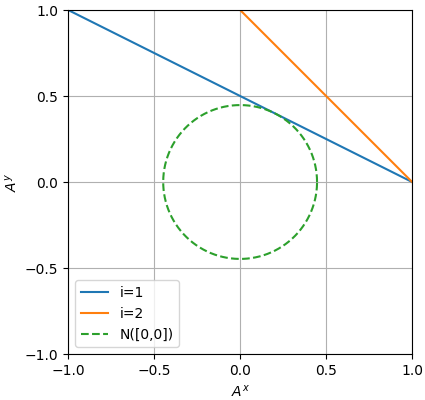
\includegraphics[width=4in]{figs/Ex.VII.1.2_fig4.png}}
    \caption{\small{The space of $\mathbf{A}\colon \mathbb{R}^2 \to \mathbb{R}$.
        Maps that fall on the solid lines map $\vec{v_i} \mapsto 1/i$.  The dashed
        green circle indicates an open neighborhood of the zero map for which
        $\mathbf{A}\vec{v_i} \ne 1/i, \forall i$, since the $i=1$ case is the most
        restrictive one. As $i$ tends to $\infty$, the radius of $N(\vec{0})|_i$,
        for which the inequality holds, tends to 1.}}
    \label{fig4}
  \end{figure}

  \newpage
  
\item[\textbf{(e)}] Deduce that $f$ has no derivative at $(0,0)$.
\item[\emph{Solution}] In order for the derivative to exist at $(0,0)$, any
  neighborhood of the zero linear map must contain a map $A$ that satisfies 
  \begin{align}
    d^\prime(f(\vec{v_i}), f(\vec{0})) = d^\prime_{f(\vec{0})}(\mathbf{D}_xf(\vec{v_i}) + \mathbf{A}\vec{v_i}).
    \label{Eqn_e}
  \end{align}
  Summarizing the prior parts of this exercise, we have:
  \begin{enumerate}[label=(\alph*), start=2, align=left]
  \item $\mathbf{D}_xf(\vec{v_i}) = 0$ for all vectors in $\mathbb{R}^2$.
  \item $d^\prime(f(\vec{v_i}), f(\vec{0})) = 1/i$ for all $i$.
  \item $\exists$ neighborhoods of the zero map for which \mathbf{A}\vec{v_i} \ne 1/i$.
  \end{enumerate}
  The existence of conditions under which Equation~\ref{Eqn_e} does not hold means
  that there is no derivative of $f$ at $(0,0)$.

  
\end{itemize}
\end{document}



%% commonly used blocks
\begin{quote}
\end{quote}

\begin{proof}
\end{proof}

\begin{align}
\end{align}

\begin{equation}
\end{equation}

\begin{remark}
\end{remark}

